\textcolor{secundario}{\gls{rfr}.} El  Flujo de ahorro en Regal\'ias se encuentra mencionado en Bolet\'in C-8 de las Mex NIF como el m\'etodo sugerido para estimar el valor razonable de activos intangibles como marcas, nombres comerciales y otros distintivos similares. Es un modelo de valuaci\'on utilizado para estimar el valor de ciertos activos intangibles  y cuenta con amplia aceptaci\'on en el medio consultor\'ia financiera (\autoref{fig:RFR}).

\begin{figure}[H]
\centering
\caption{Objeto del modelo RFR\label{fig:RFR}}
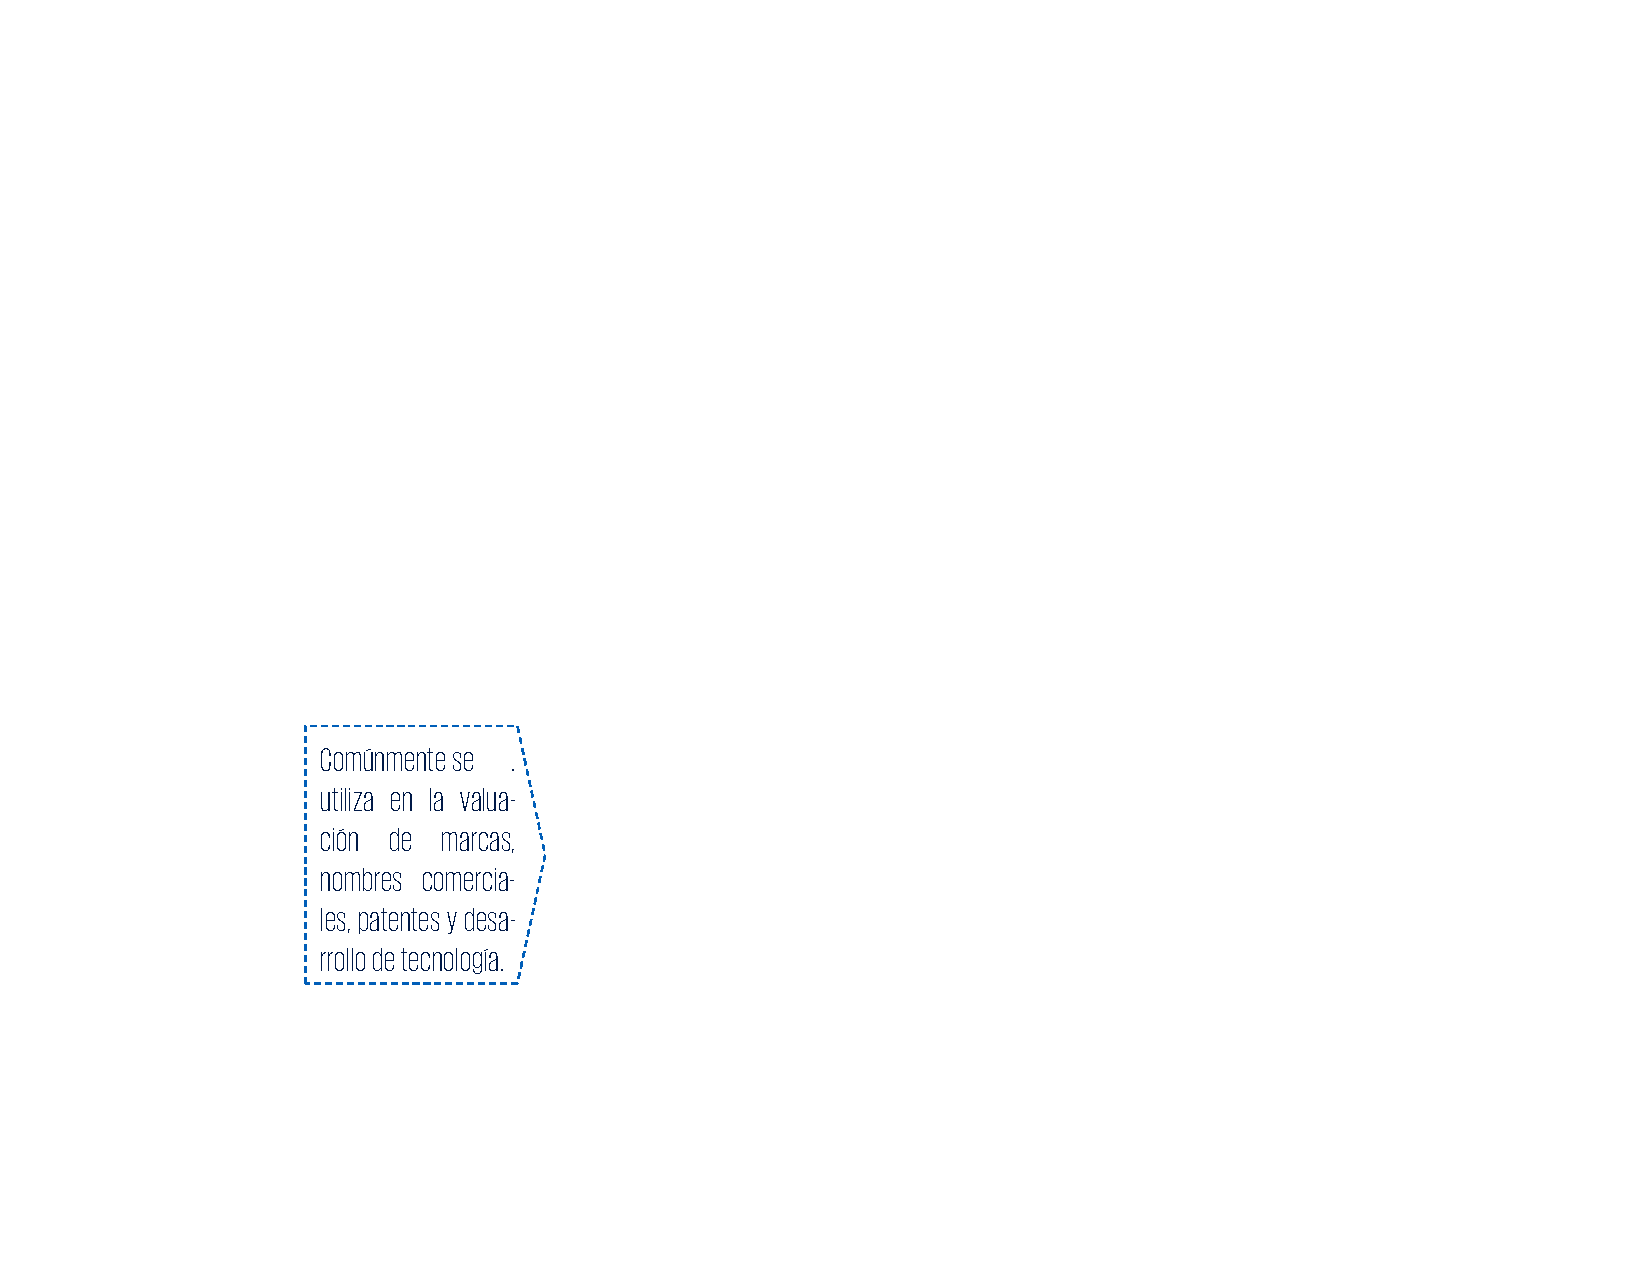
\includegraphics[width=4cm]{\rutaImagenes/RFR}\\
\end{figure}

\textbf{\textcolor{principal}{Aplicaci\'on del m\'etodo.}} Este modelo involucra la estimaci\'on del valor justo de un activo intangible, cuantificando el valor presente del flujo de pagos de regal\'ias que el propietario del activo intangible est\'a exento (\autoref{fig:RFR_2}). Se basa en la premisa de que el \'unico valor que el comprador de un activo intangible recibe es el ahorro por no tener que pagar regal\'ias a un tercero por el uso de dicho activo.

\begin{figure}[H]
\centering
\caption{Premisas del modelo RFR\label{fig:RFR_2}}
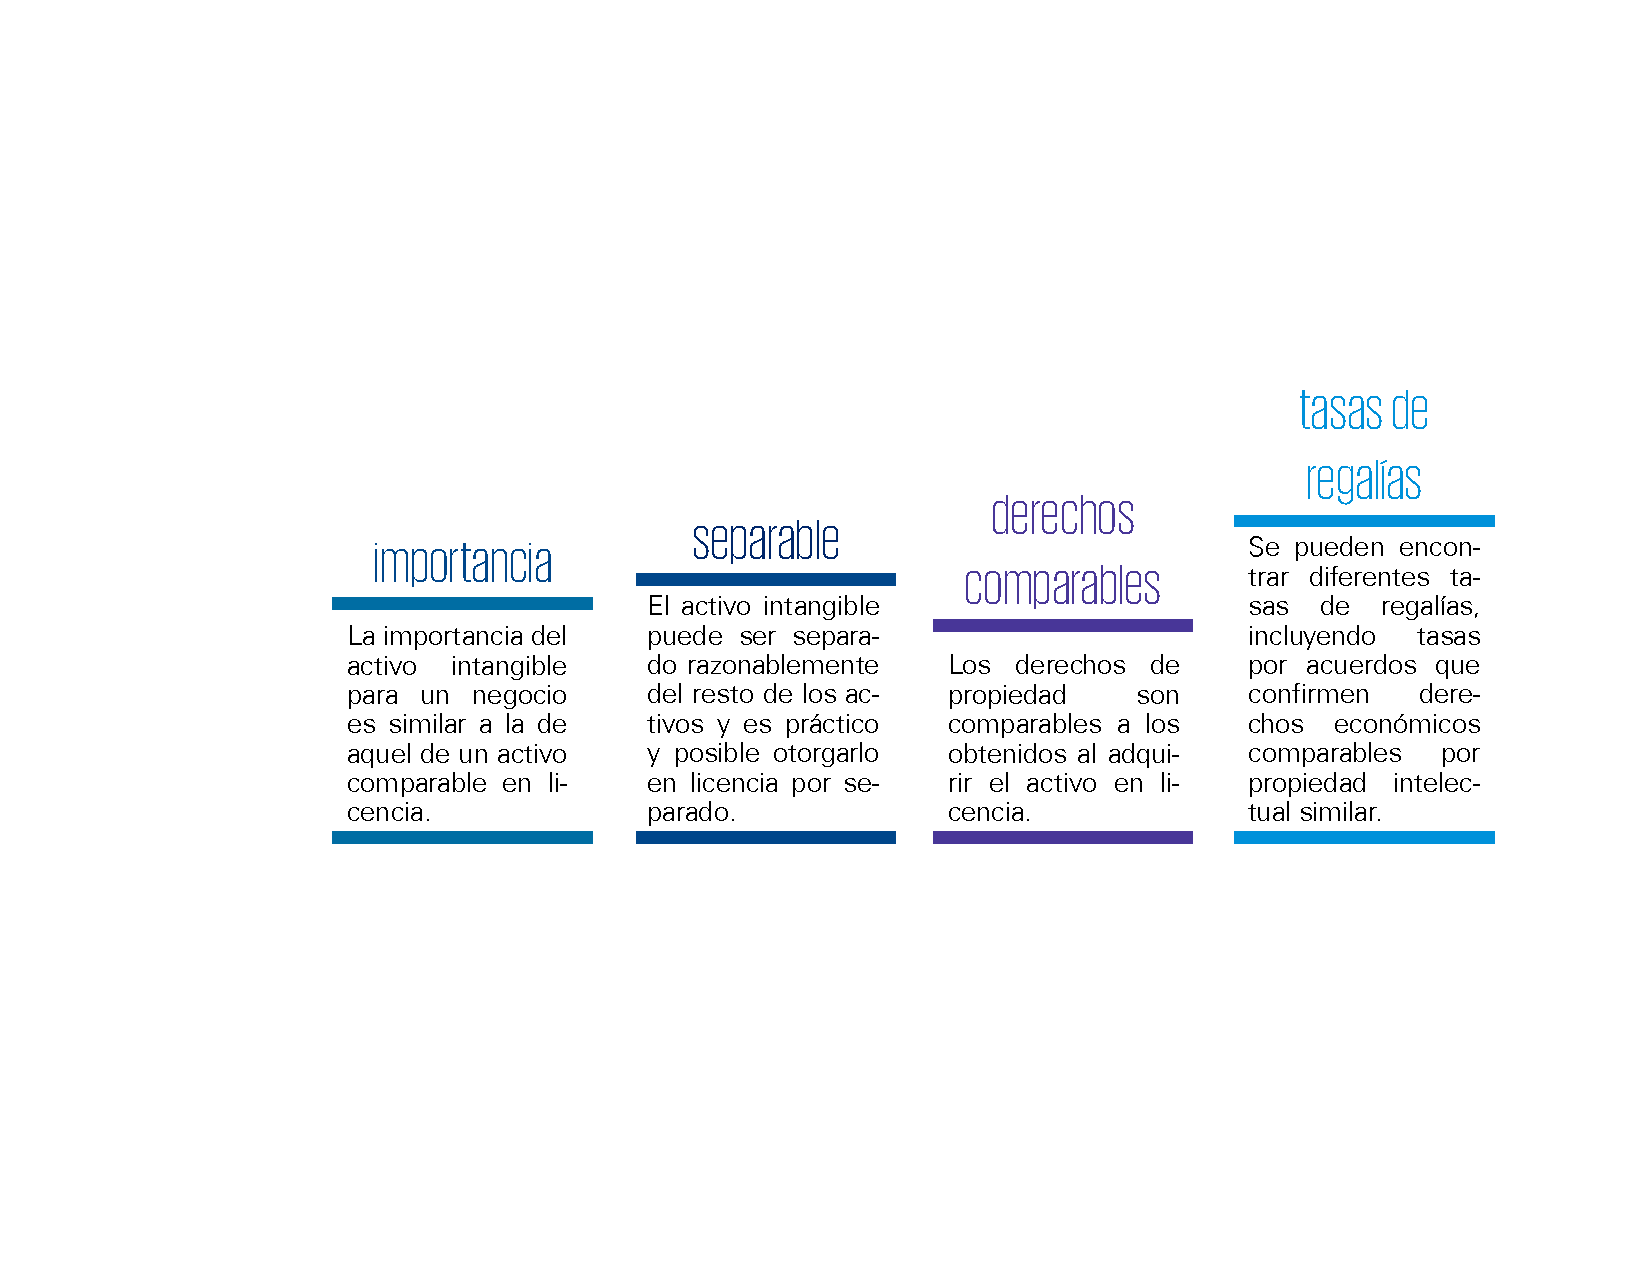
\includegraphics[width=10cm]{\rutaImagenes/RFR_2}\\
\end{figure}